%!TEX program = xelatex
\documentclass[dvipsnames, svgnames,a4paper,11pt]{article}
% ----------------------------------------------------- 
%	加边框的命令
%	参考:https://tex.stackexchange.com/questions/531559/how-to-add-the-page-border-for-first-two-pages-in-latex
\usepackage{tikz}
\usetikzlibrary{calc}
\usepackage{eso-pic}
\AddToShipoutPictureBG{%
\begin{tikzpicture}[overlay,remember picture]
\draw[line width=0.6pt] % 边框粗细
    ($ (current page.north west) + (0.6cm,-0.6cm) $)
    rectangle
    ($ (current page.south east) + (-0.6cm,0.6cm) $); % 边框位置
\end{tikzpicture}}


\usepackage{xcolor}
\definecolor{c1}{HTML}{086173} % 目录颜色 原版为2752C9 紫灰色535AAA 蓝紫色0B0DB7 深蓝色070F94 湖绿色219394 松石灰绿086173
\definecolor{c2}{HTML}{E20129} % 引用颜色 原版\definecolor{c2}{RGB}{190,20,83} 橙色F24729

\usepackage{ctex}
\usepackage[top=28mm,bottom=28mm,left=15mm,right=15mm]{geometry}
\usepackage{hyperref} 
\hypersetup{
	colorlinks,
	linktoc = section, % 超链接位置,选项有section, page, all
	linkcolor = c1, % linkcolor 目录颜色
	citecolor = c1  % citecolor 引用颜色
}
\usepackage{amsmath,enumerate,multirow,float}
\usepackage{tabularx}
\usepackage{tabu}
\usepackage{subfig}
\usepackage{fancyhdr}
\usepackage{graphicx}
\usepackage{wrapfig}  
\usepackage{physics}
\usepackage{appendix}
\usepackage{amsfonts}

%
\usepackage{tcolorbox}
\tcbuselibrary{skins,breakable}
\newtcolorbox{tbox}[2][]{
    colframe=black!70!,
    breakable,
    enhanced,
	boxrule =0.5pt,
    title = {#2},
    fonttitle = \large\kaishu\bfseries,
	drop fuzzy shadow,
    #1
}
\newtcolorbox[auto counter,number within=section]{question}[1][]{
  top=2pt,bottom=2pt,arc=1mm,
  boxrule=0.5pt,
%   frame hidden,
  breakable,
  enhanced, %跨页后不会显示下边框
  coltitle=c1!80!gray,
  colframe=c1,
  colback=c1!3!white,
  drop fuzzy shadow,
  title={思考题~\thetcbcounter:\quad},
  fonttitle=\bfseries,
  attach title to upper,
  #1
}

% ---------------------------------------------------------------------
%	利用cleveref改变引用格式,\cref是引用命令
\usepackage{cleveref}
\crefformat{figure}{#2{\textcolor{c2}{Figure #1}}#3} % 图片的引用格式
\crefformat{equation}{#2{(\textcolor{c2}{#1})}#3} % 公式的引用格式
\crefformat{table}{#2{\textcolor{c2}{Table #1}}#3} % 表格的引用格式


% ---------------------------------------------------------------------
%	页眉页脚设置
\fancypagestyle{plain}{\pagestyle{fancy}}
\pagestyle{fancy}
\lhead{\kaishu 中山大学物理与天文学院电子技术实验\uppercase\expandafter{\romannumeral1}} % 左边页眉,学院 + 课程
\rhead{\kaishu 实验报告By黄罗琳} % 右边页眉,实验报告标题
\cfoot{\thepage} % 页脚,中间添加页码


% ---------------------------------------------------------------------
%	对目录、章节标题的设置
\renewcommand{\contentsname}{\centerline{\huge 目录}}
\usepackage{titlesec}
\usepackage{titletoc}
% \titleformat{章节}[形状]{格式}{标题序号}{序号与标题间距}{标题前命令}[标题后命令]
\titleformat{\section}{\centering\LARGE\songti}{}{1em}{}

% ---------------------------------------------------------------------
%   listing代码环境设置
\usepackage{listings}
\lstloadlanguages{python}
\lstdefinestyle{pythonstyle}{
backgroundcolor=\color{gray!5},
language=python,
frameround=tftt,
frame=shadowbox, 
keepspaces=true,
breaklines,
columns=spaceflexible,                   
basicstyle=\ttfamily\small, % 基本文本设置,字体为teletype,大小为scriptsize
keywordstyle=[1]\color{c1}\bfseries, 
keywordstyle=[2]\color{Red!70!black},   
stringstyle=\color{Purple},       
showstringspaces=false,
commentstyle=\ttfamily\scriptsize\color{green!40!black},%注释文本设置,字体为sf,大小为smaller
tabsize=2,
morekeywords={as},
morekeywords=[2]{np, plt, sp},
numbers=left, % 代码行数
numberstyle=\it\tiny\color{gray}, % 代码行数的数字字体设置
stepnumber=1,
rulesepcolor=\color{gray!30!white}
}




% ---------------------------------------------------------------------
%	其他设置
\def\degree{${}^{\circ}$} % 角度
\graphicspath{{./images/}} % 插入图片的相对路径
\allowdisplaybreaks[4]  %允许公式跨页 
\usepackage{lipsum}
\usepackage{adjustbox}
\usepackage{multirow}
\usepackage{amsmath}

%\usepackage{mathrsfs} % 字体
%\captionsetup[figure]{name=Figure} % 图片形式
%\captionsetup[table]{name=Table} % 表格形式
\begin{document}
	
	% 实验报告封面	
	% 顶栏
	\begin{table}
		\renewcommand\arraystretch{1.7}
		\begin{tabularx}{\textwidth}{
				|X|X|X|X
				|X|X|X|X|}
			\hline
			\multicolumn{2}{|c|}{预习报告}&\multicolumn{2}{|c|}{实验记录}&\multicolumn{2}{|c|}{分析讨论}&\multicolumn{2}{|c|}{总成绩}\\
			\hline
			\LARGE25 & & \LARGE25 & & \LARGE30 & & \LARGE80 & \\
			\hline
		\end{tabularx}
	\end{table}
	% ---
	
	% 信息栏
	\begin{table}
		\renewcommand\arraystretch{1.7}
		\begin{tabularx}{\textwidth}{|X|X|X|X|}
			\hline
			年级、专业: & 2022级 物理学 &组号: &D8 \\
			\hline
			姓名: & 黄罗琳、王显   & 学号: &  22344001、22344002 \\
			\hline
			实验时间: & 2024/4/10 & 教师签名: & \\
			\hline
		\end{tabularx}
	\end{table}
	% ---
	
	% 大标题
	\begin{center}
		\LARGE ET6  \quad R、L、C元件阻抗特性研究
	\end{center}
	% ---
	
	% 注意事项
	
	% 基本
	\textbf{【实验报告注意事项】}
	\begin{enumerate}
		\item 实验报告由三部分组成:
		\begin{enumerate}
			\item 预习报告:课前认真研读实验讲义,弄清实验原理;实验所需的仪器设备、用具及其使用、完成课前预习思考题;了解实验需要测量的物理量,并根据要求提前准备实验记录表格(可以参考实验报告模板,可以打印)。\textcolor{red}{\textbf{(20分)}}
			\item 实验记录:认真、客观记录实验条件、实验过程中的现象以及数据。实验记录请用珠笔或者钢笔书写并签名(\textcolor{red}{\textbf{用铅笔记录的被认为无效}})。\textcolor{red}{\textbf{保持原始记录,包括写错删除部分,如因误记需要修改记录,必须按规范修改。}}(不得输入电脑打印,但可扫描手记后打印扫描件);离开前请实验教师检查记录并签名。\textcolor{red}{\textbf{(30分)}}
			\item 数据处理及分析讨论:处理实验原始数据(学习仪器使用类型的实验除外),对数据的可靠性和合理性进行分析;按规范呈现数据和结果(图、表),包括数据、图表按顺序编号及其引用;分析物理现象(含回答实验思考题,写出问题思考过程,必要时按规范引用数据);最后得出结论。\textcolor{red}{\textbf{(30分)}}
		\end{enumerate}
		\textbf{实验报告就是将预习报告、实验记录、和数据处理与分析合起来,加上本页封面。\textcolor{red}{(80分)}}
	
	\end{enumerate}
		
	
	% 安全
	\textbf{【实验安全注意事项】}	
	\begin{enumerate}
		\item 采用万用表交流电压档测量交流电压时,请注意有效频率范围。
		\item 在使用示波器测量电压或相位差时,注意示波器两个通道输入信号的接地点接法必须保证信号源、示波器所有通道的接地点接在电路的同一个点上。
		\item 在使用示波器测量电压或相位差时,示波器输入信号的耦合方式要选择交流耦合。
		\item 绘制幅频特性和相频特性曲线时,频率轴采用对数坐标。
		\item 在计算时请注意角频率与频率的转换。
	\end{enumerate}
	
	% 目录
	\clearpage
	\tableofcontents
	\clearpage
	% ---
	
	
	
	% 预习报告	
	
	% 小标题
	\setcounter{section}{0}
	\section{ET6 R、L、C元件阻抗特性研究\quad\heiti 预习报告}
	% ---
	
	% 实验目的
	\subsection{实验目的}
	\begin{enumerate}
		\item[1.] 测量电阻、感抗、容抗与频率的关系,测定 $R$-$f$、$X_L$-$f$ 及 $X_C$-$f$ 特性曲线。
		\item[2.] 观察并了解 $R$、$L$、$C$ 元件两端电压与电流间的相位关系。
	\end{enumerate}
	% ---
	
	% 仪器用具
	\subsection{仪器用具}
	\begin{table}[htbp]
		\centering
		\renewcommand\arraystretch{1.6}
		\begin{tabular}{|c|p{3cm}|c|p{5cm}|c|p{2cm}|}
			\hline
			序号 & 名称 & 型号 & 技术特性及说明 & 数量 & 备注 \\
			\hline
			1 & 电路原理箱或板 & & & 1 & \\
			2 & 函数信号发生器 & DG4162& & 1 & \\
			3 & 交流毫伏表 & & & 1 & \\
			4 & 直流电压表或万用表 &  & 0~30V& 1 & \\
			5 & 2号实验导线 & & 二端2号镀金插头 & N & \\
			\hline
		\end{tabular}
	\end{table}
	

	% ---
	
	% 原理概述
	\subsection{原理概述}
	\subsubsection{元件阻抗表达式}
阻抗 \( Z \) 是电路中元件对交流信号的阻碍程度,对于电阻 \( R \),阻抗是恒定的,为其本身的阻值。对于电感 \( L \) 和电容 \( C \),阻抗与信号频率有关。$\text{电感的复阻抗为 }Z_L=j\omega L\text{,电容的复阻抗为 }Z_C=\frac1{j\omega C}。$
\begin{table}[htbp]
	\centering
	\caption{R、L、C元件阻抗表达式}
	\begin{tabular}{|c|c|c|c|c|}
		\hline
	  元件 & 阻抗表达式 & 元件 & 阻抗表达式 \\ 
	  \hline
	  电阻 \( R \) & \( R \) & 电感 \( L \) & $Z_{L}=j\omega L$ \\
	  \hline
	  电容 \( C \) & $Z_C=\frac{1}{j\omega C}$ & 总阻抗 \( Z \) & \( Z = R + j(Z_L - Z_C) \) \\ 
	  \hline
	\end{tabular}
  \end{table}
\subsubsection{幅频特性与相频特性}
幅频特性曲线描述了电路中电压幅值随频率变化的关系。通过保持输入电压幅值恒定,并改变信号频率,可以绘制出电抗元件在串联电路中电压与频率的关系曲线。相频特性曲线描述了阻抗角(相位差)随频率变化的关系。相位差 \( \phi \) 可以通过双踪示波器测量,根据波形周期和相位差的关系计算得到。

\subsubsection{电压向量三角形与阻抗三角形}
电压向量三角形是指输入电压向量与电抗元件电压向量以及串联电阻电压向量之间的关系。根据三角形相似性原理,这三个电压向量所组成的三角形与整个电路的阻抗三角形相似。电压向量之间的相位关系决定了电压向量三角形的形状和大小,而阻抗三角形则反映了整个电路中各个元件的阻抗相互关系。

通过测量电压和相位差随频率的变化,可以得到电路的幅频特性曲线和相频特性曲线,从而全面了解 \( R \)、 \( L \)、 \( C \) 元件在交流电路中的行为特性。

	% ---
	
	
	
	% 实验前思考题
	\subsection{实验预习题}
	
	% 思考题1
	\begin{question}
		正弦稳态电路中采用向量法简化计算;
	\end{question}
	\begin{itemize}
		\item \textbf{复数表示}:
		  \begin{itemize}
			\item 将正弦波形的电压、电流等参数表示为复数形式。
			\item 例如,一个电压 $V = V_m \sin(\omega t + \phi)$ 可以表示为复数形式 $\hat{V} = V_m e^{j\phi}$,其中 $\hat{V}$ 是电压的复数形式,$V_m$ 是电压幅值,$\phi$ 是相位角,$j$ 是虚数单位。
		  \end{itemize}
		  
		\item \textbf{复数运算}:
		  \begin{itemize}
			\item 在复数形式下,电路中的各种元件(电阻、电感、电容等)都可以用复阻抗来表示。
			\item 电感的复阻抗为 $Z_L = j\omega L$,电容的复阻抗为 $Z_C = \frac{1}{j\omega C}$。
		  \end{itemize}
		  
		\item \textbf{求解电路参数}:
		  \begin{itemize}
			\item 根据电路中各个元件的复阻抗以及复数形式下的欧姆定律和基尔霍夫定律,可以求解电路中各个节点的电压、电流等参数。
			\item 通过相量法的简化计算,可以更快地得到电路的稳态响应,并且能够直观地理解电路中各个参数之间的关系。
		  \end{itemize}
	  \end{itemize}
	% 思考题2
	\begin{question}
		时域和频域表达方式的互相转换.
	\end{question}
	\subsection*{从时域到频域:}
\begin{itemize}
  \item 时域信号函数 $x(t)$ 可以通过傅里叶变换表示为频域的形式 $X(f)$,用以分析信号的频率成分。
  \item 傅里叶变换公式为:
    \[
    X(f) = \int_{-\infty}^{\infty} x(t)e^{-j2\pi ft} dt
    \]
  \item 其中,$X(f)$ 是频率为 $f$ 的信号成分的复幅值,$f$ 是频率,$j$ 是虚数单位。
\end{itemize}

\subsection*{从频域到时域:}
\begin{itemize}
  \item 频域的信号函数 $X(f)$ 可以通过逆傅里叶变换表示为时域的形式 $x(t)$,还原出原始信号。
  \item 逆傅里叶变换公式为:
    \[
    x(t) = \int_{-\infty}^{\infty} X(f)e^{j2\pi ft} df
    \]
  \item 其中,$x(t)$ 是时域信号函数,$X(f)$ 是频域信号的复幅值。
\end{itemize}
	
	% 思考题3
	\begin{question}
		阻抗三角形、电压向量三角形和功率三角形;
	\end{question}
	\begin{figure}[{H}]
		\centering
		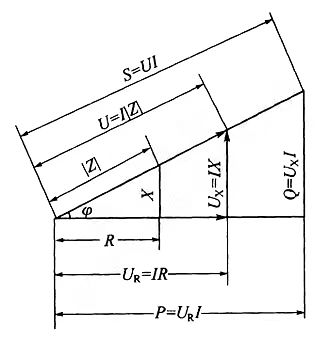
\includegraphics[width=0.4\linewidth]{原理三角形.jpg}
		\caption{三种三角形相似}
		\label{}
	\end{figure}
	\subsection*{阻抗三角形:}
	阻抗三角形是指在交流电路中,由电阻、电感和电容组成的三角形,其中各边分别代表电阻、电感和电容的阻抗。根据电路中的阻抗关系,阻抗三角形的任意两边之和等于第三边,符合基尔霍夫定律。
	
	\subsection*{电压向量三角形:}
	电压向量三角形是指在交流电路中,输入电压、电抗元件上的电压和串联电阻上的电压所组成的三角形。根据电路中的电压关系,电压向量三角形的任意两边之和等于第三边,符合基尔霍夫定律。
	
	\subsection*{功率三角形:}
	功率三角形是指在交流电路中,输入功率、有功功率和无功功率所组成的三角形。根据电路中的功率关系,功率三角形的任意两边之和等于第三边,符合功率平衡定律。
	


	\begin{question}
		RC和RL电路的频率特性分析;
	\end{question}
	\subsection*{RC电路的频率特性分析:}
RC电路是由电阻(R)和电容(C)组成的电路。其频率特性分析涉及电压、电流的相位和幅值随频率的变化。
\begin{itemize}
  \item 幅频特性:在RC电路中,随着频率的增加,电容的阻抗减小,导致整体电路的阻抗减小,电压幅值增加。频率越高,电压幅值越大。
  \item 相频特性:RC电路的相位差随频率的变化呈线性变化,相位差随频率增大而增加,最终趋向于90度。
\end{itemize}

\subsection*{RL电路的频率特性分析:}
RL电路是由电阻(R)和电感(L)组成的电路。其频率特性分析同样涉及电压、电流的相位和幅值随频率的变化。
\begin{itemize}
  \item 幅频特性:在RL电路中,随着频率的增加,电感的阻抗增大,导致整体电路的阻抗增大,电压幅值减小。频率越高,电压幅值越小。
  \item 相频特性:RL电路的相位差随频率的变化呈线性变化,相位差随频率增大而减小,最终趋向于0度。
\end{itemize}
	% ---
	
	
	
	% 实验记录	
	\clearpage
	
	% 顶栏
	\begin{table}
		\renewcommand\arraystretch{1.7}
		\centering
		\begin{tabularx}{\textwidth}{|X|X|X|X|}
			\hline
			专业: & 物理学 & 年级: & 2022级 \\
			\hline
			姓名: &黄罗琳、王显  & 学号: &22344001、22344002 \\
			\hline
			室温: &23℃  & 实验地点: & A522 \\
			\hline
			学生签名:&
\includegraphics[width=1cm]{签字.jpg} 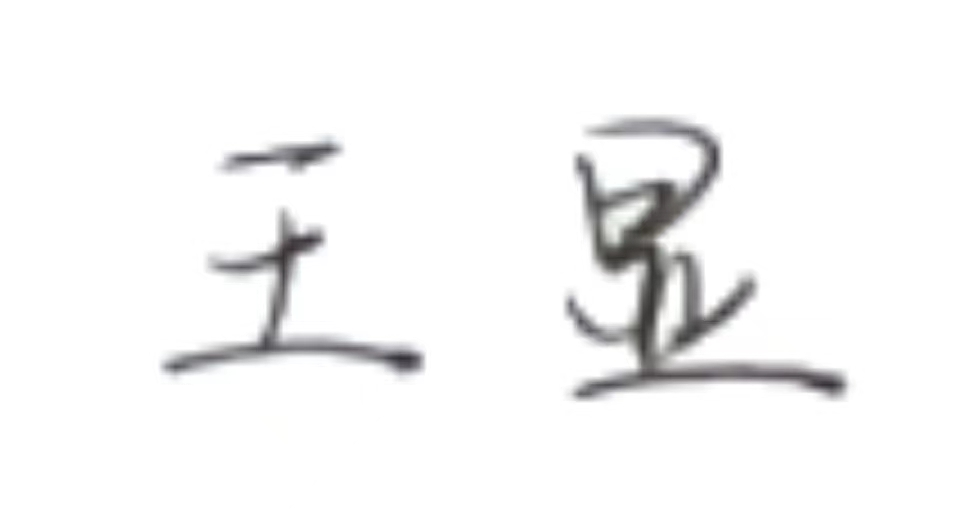
\includegraphics[width=1cm]{wx.jpg}   & 评分: &\\
			\hline
			实验时间:& 2024/4/10 & 教师签名:&\\
			\hline
		\end{tabularx}
	\end{table}
	% ---
	
	% 小标题
	\section{ET6 R、L、C元件阻抗特性研究 \quad\heiti 实验记录}
	% ---
	
	% 实验过程记录
	\subsection{实验内容、步骤与结果}
	
	%
	\subsubsection{测量R、L、C元件的阻抗频率特性}
	\begin{enumerate}
		\item 实验电路图如下:
		\begin{figure}[{H}]
			\centering
			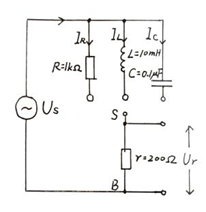
\includegraphics[width=0.4\linewidth]{电路图.png}
			\caption{实验电路图}
			\label{}
		\end{figure}
		
		
		
		\item 通过函数信号发生器输出正弦信号接至如图所示电路,作为激励源$U_S$,并用台式万用表交流电压档或示波器测量,激励电压设置为正弦信号输出,无直流偏置,有效值$U_{RMS}=3V$,并在实验过程中保持不变。
		
		使信号源的输出频率从100Hz逐渐增至100KHz左右, 并使端点S分别接通R、L、C三个元件,分别测量UR、Ur,UL、Ur,Uc、Ur,并通过计算得到各频率点时的R、XL与Xc之值。

		用双踪示波器观察$R_L$串联和$R_C$串联电路在不同频率下阻抗角的变化情况。
		\\\textbf{实验数据记录为有效值,示波器通过光标测量为峰峰值,通过计算后得出有效值并记录在表格中。}
		\item 实验数据:
		\begin{table}[h]
			\centering
			\begin{tabular}{|c|c|c|c|c|}
			\hline
			$f(KHZ)$ & $U_r(V)$ & $U_R(V)$ & $R(\Omega)$ & $\phi °$ \\
			\hline
			
			100   & 0.505 & 2.495 & 988.1188119 & $0 $\\
			
			50  & 0.507 & 2.493 & 983.4319527 &$0 $\\
		
			20   & 0.504 & 2.496 & 990.4761905 & $0 $\\
			
			10  & 0.505 & 2.495 & 988.1188119 &$0 $ \\
			
			5   & 0.505 & 2.495 & 988.1188119 &$0 $ \\
			
			2   & 0.505 & 2.495 & 988.1188119 & $0 $\\
			
			1   & 0.505 & 2.495 & 988.1188119 & $0 $\\
			
			0.5   & 0.506 & 2.494 & 985.770751 & $0 $\\
			
			0.2   & 0.504 & 2.496 & 990.4761905 & $0 $\\
			
			0.1   & 0.505 & 2.495 &988.1188119 &$0 $ \\
		\hline
			
			\end{tabular}
			\caption{R元件阻抗实验数据}
			
			\end{table}
			\begin{table}[H]
				\centering
				\begin{tabular}{|c|c|c|c|c|}
					\hline
					$f (kHz)$ & $U_r (V)$ &$ U_L (V)$ & $X_L$& 角度 (°) \\
					\hline
					0.1  & 3.00 & 0.02 & 1.33 & 0.19 \\
					0.2  & 3.00 & 0.03 & 2.00 & 0.46 \\
					0.5  & 2.99 & 0.08 & 5.35 & 1.28 \\
					1    & 2.98 & 0.15 & 10.07 & 2.58 \\
					2    & 2.98 & 0.27 & 18.12 & 5.67 \\
					5    & 2.91 & 0.70 & 48.11 & 13.91 \\
					10   & 2.71 & 1.27 & 93.54 & 25.81 \\
					20   & 2.13 & 2.12 & 199.53 & 44.73 \\
					50   & 1.18 & 2.75 & 466.10 & 67.45 \\
					100  & 0.62 & 2.94 & 948.39 & 77.68 \\
					\hline
				\end{tabular}
				\caption{电感阻抗实验数据}
			\end{table}

				\begin{table}[h]
					\centering
					\begin{tabular}{|c|c|c|c|c|}
						\hline
						分压比 & 频率 (Hz) & $U_r (V)$ & $U_L (V)$ & $\phi °$ \\
						\hline
						1:1 & 20k & 2.13 & 2.12 & 44.73 \\
						1:2 & 40k & 1.35 & 2.65 & 62.87 \\
						2:1 & 10k & 2.70 & 1.33 & 28.08 \\
						\hline
					\end{tabular}
					\caption{不同分压比($U_r $/$U_L $)实验数据}
				\end{table}
				\begin{table}[H]
					\centering
					\begin{tabular}{|c|c|c|c|c|}
						\hline
						$f (Hz)$ & $U_r (V)$ & $U_C (V)$ & $X_C$ & Ψ (°) \\
						\hline
						100      & 0.01  & 3.00  & 60000.00 & -89.88 \\
						200      & 0.01  & 3.00  & 60000.00 & -89.78 \\
						500      & 0.03  & 3.00  & 20000.00 & -89.45 \\
						1k       & 0.07  & 3.00  & 8571.43  & -88.89 \\
						2k       & 0.13  & 2.99  & 4600.00  & -87.76 \\
						5k       & 0.31  & 2.98  & 1922.58 & -84.32 \\
						10k      & 0.60  & 2.95  & 983.33  & -78.82 \\
						20k      & 1.13  & 2.77  & 489.73 & -68.28 \\
						50k      & 2.12  & 2.09  & 197.17 & -45.23 \\
						100k     & 2.69  & 1.34  & 99.62 & -26.72 \\
						200k     & 2.94  & 0.75  & 51.02  & -14.12 \\
						\hline
					\end{tabular}
					\caption{电容阻抗实验数据}
				\end{table}
				\begin{table}[H]
					\centering
					\begin{tabular}{|c|c|c|c|c|}
						\hline
						分压比 & 频率 (Hz) & Ur (V) & Uc (V) & Ψ (°) \\
						\hline
						1:1   & 50k       & 2.12  & 2.09  & -45.73 \\
						1:2   & 25k       & 1.34  & 2.68  & -64.15 \\
						2:1   & 100k      & 2.69  & 1.34  & -25.72 \\
						\hline
					\end{tabular}
					\caption{不同分压比($U_r $/$U_C $)实验数据}
				\end{table}
	\end{enumerate}	
	
	%
	\subsubsection{测量出该电感内部包含的自有电阻$R_L$}
	\begin{enumerate}
		\item 方法一:
		直接法

		直接将欧姆表连接在电感两端,所测得数值为$25.65\Omega$
		\item 方法二:串联谐振测量法
		
	    相关实验原理见分析与讨论,如图所示连接电路
		\begin{figure}[{H}]
			\centering
			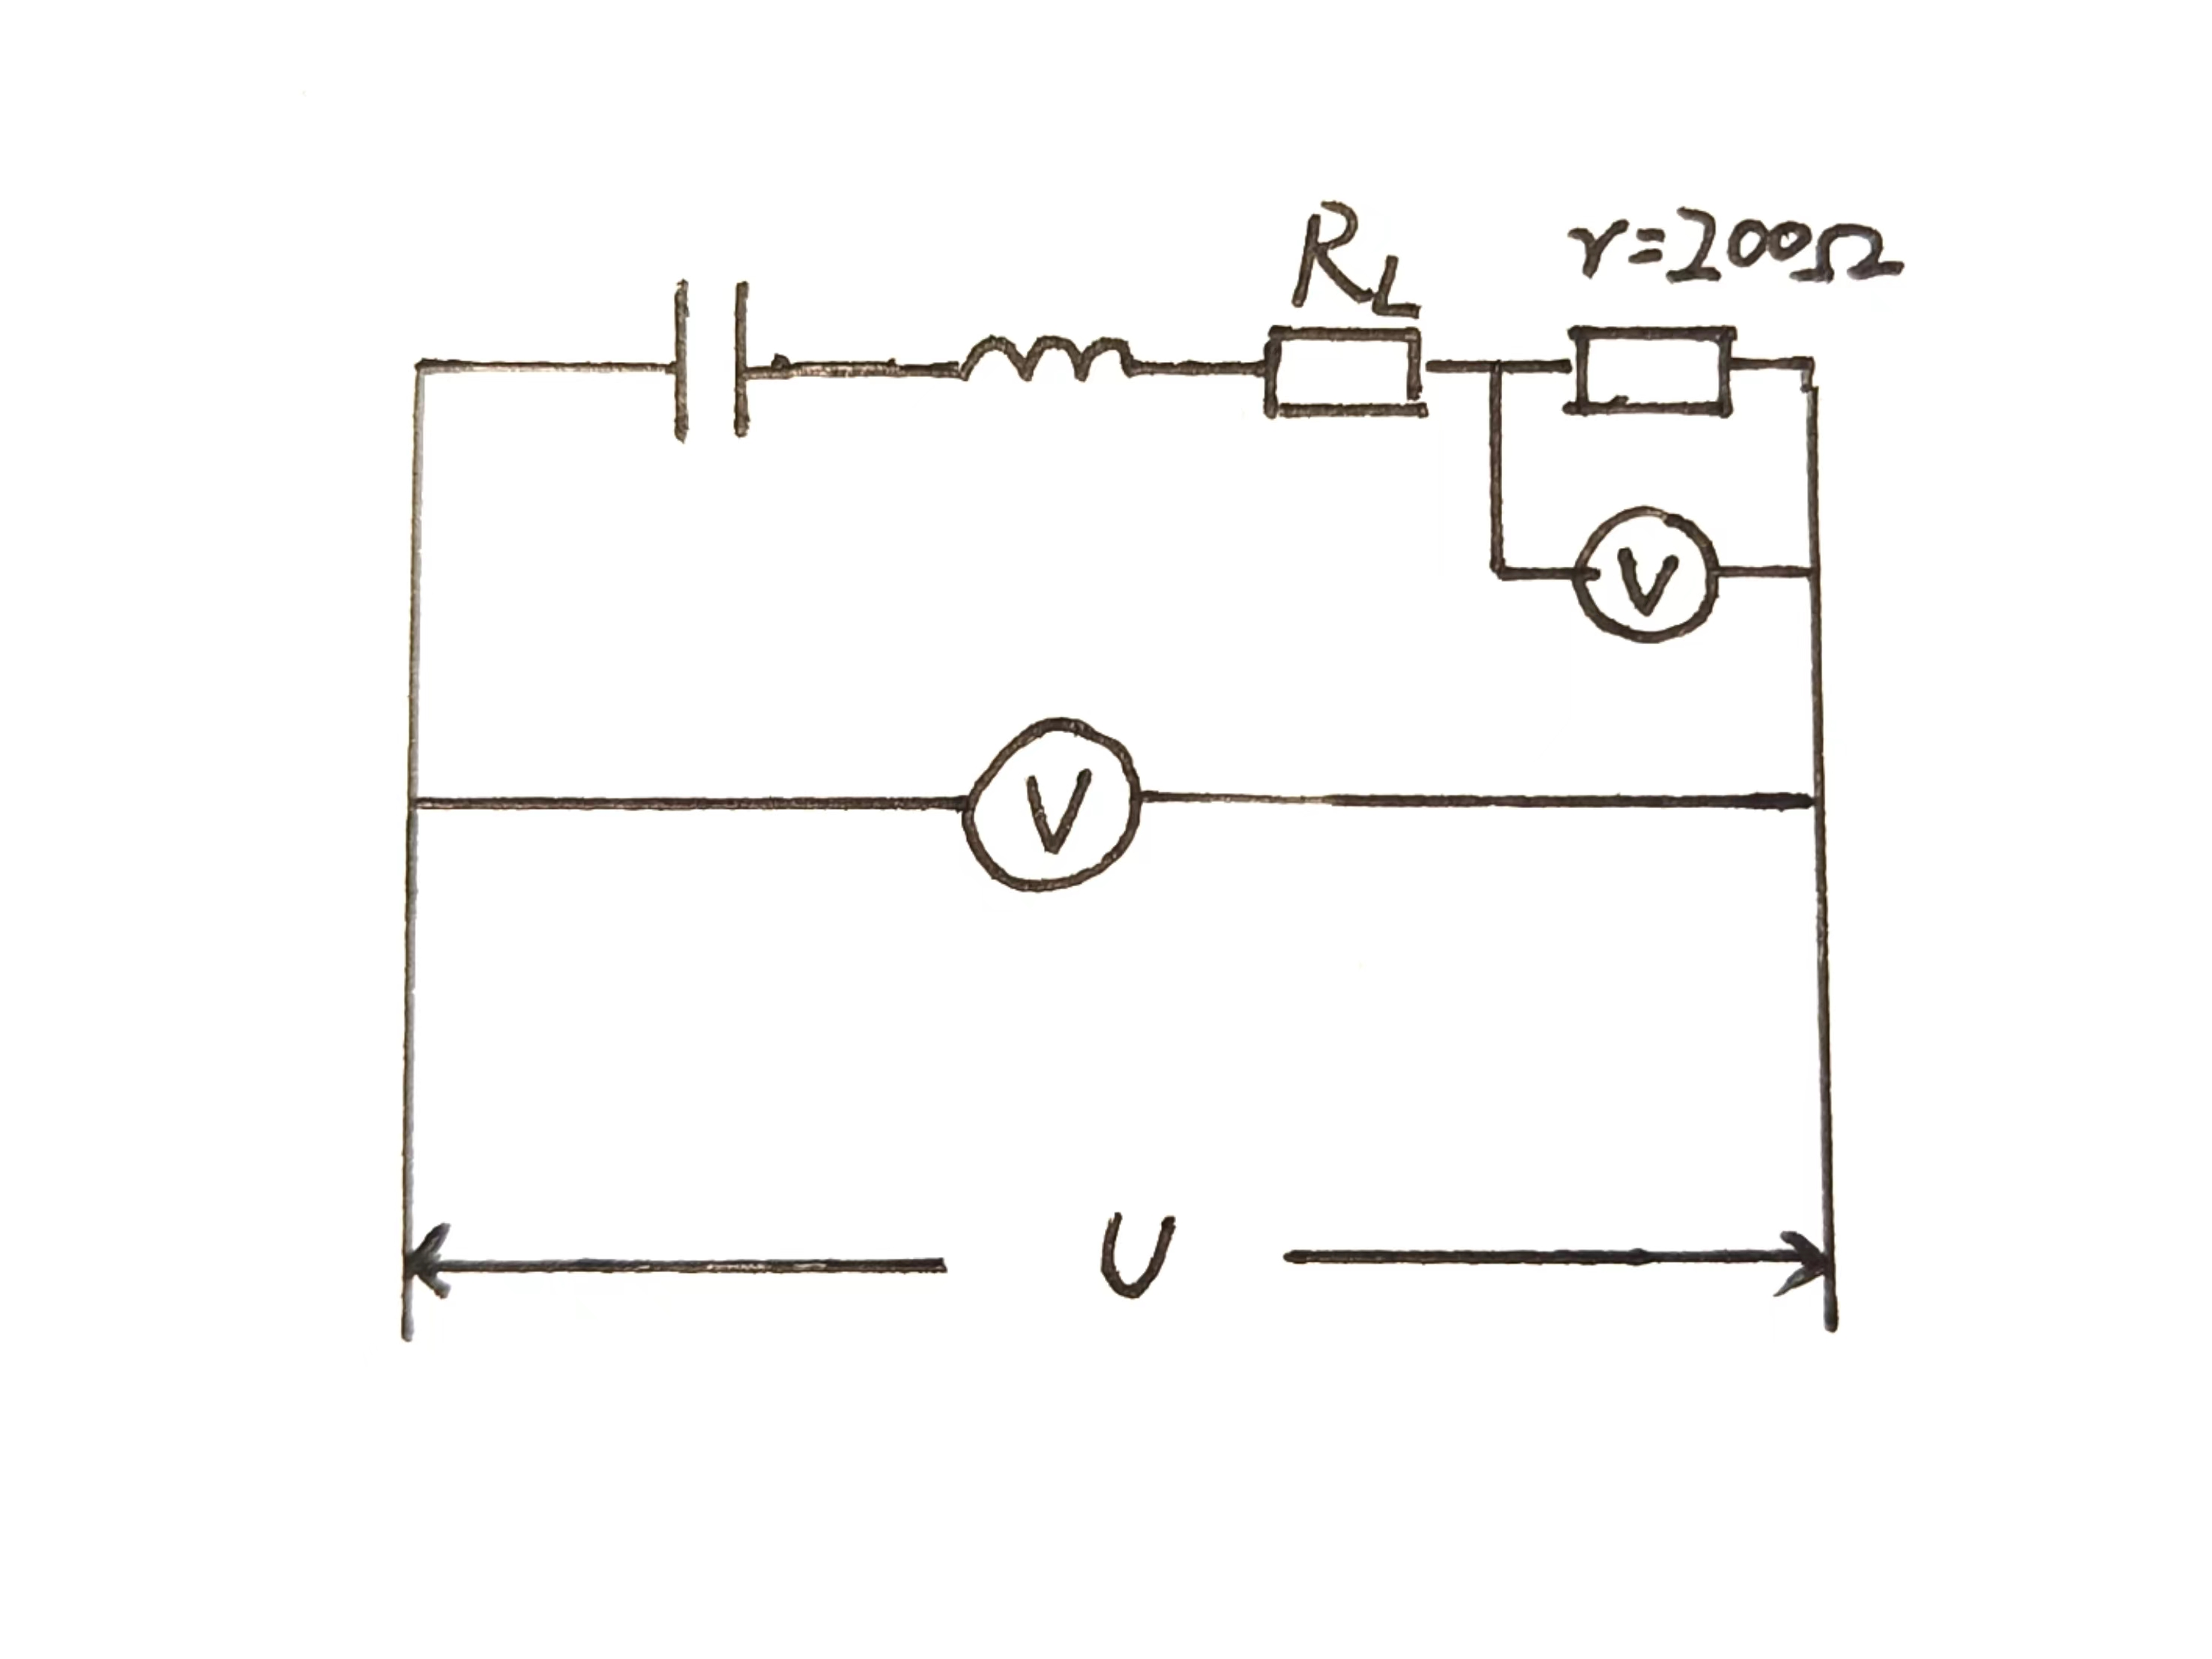
\includegraphics[width=0.4\linewidth]{电路2.jpg}
			\caption{测量电路图}
			\label{}
		\end{figure}

		$U_{总}=2.207V$\quad$U_r=1.920V$  $$f_{\mathrm{r}}=\frac1{2\pi\sqrt{\mathrm{LC}}}=5035HZ$$
		
		
	计算所得$R_L=27.97\Omega$
	\end{enumerate}
	
	% ---
	
	% 原始数据
	
	% 问题记录
	\subsection{实验过程遇到问题及解决办法}
	
		在实验过程中,起初并没有接入电压表对电源电压进行监测,尽管信号源的输出电压屏幕显示为3V,但是实际上根据一系列不符合理论计算的实验结果说明,信号源的输出电压出现了改变,之后通过接入一个台式万用表对示波器的输出电压进行监测,然后保证不同频率下调整屏幕显示输出电压保证万用表测量电压为3V,得到了正确的实验结果。
	
	% ---
	
	
	
	% 分析与讨论	
	\clearpage
	
	% 顶栏
	\begin{table}
		\renewcommand\arraystretch{1.7}
		\begin{tabularx}{\textwidth}{|X|X|X|X|}
			\hline
			专业:& 物理学 &年级:& 2022级\\
			\hline
			姓名: &黄罗琳、王显  & 学号:&22344001、22344002 \\
			\hline
			日期:& 2024/4/10 & 评分: &\\
			\hline
		\end{tabularx}
	\end{table}
	% ---
	
	% 小标题
	\section{ET6 R、L、C元件阻抗特性研究\quad\heiti 分析与讨论}
	% ---
	
	% 数据处理
	\subsection{RC电路分析}
	\subsubsection{幅频关系曲线}
	根据实验数据,绘制幅频关系曲线
\begin{figure}[{H}]
	\centering
	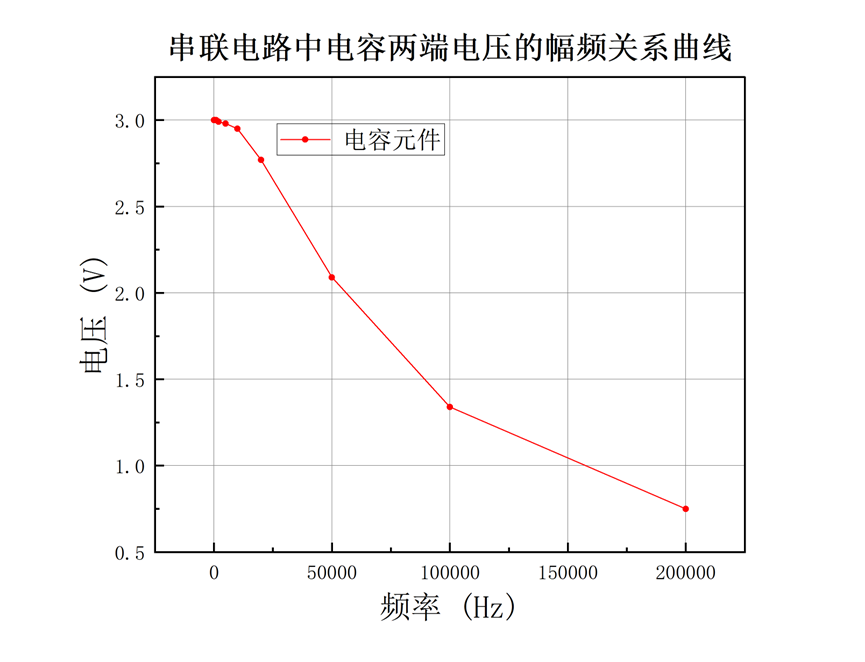
\includegraphics[width=0.55\linewidth]{c.png}

	\label{}
\end{figure}
\textbf{图像分析:}

在RC串联电路中,电容和电阻串联连接,输入电压施加到整个电路上。电容的阻抗是频率的函数,阻抗 \( Z_C \) 的表达式为:

\[
Z_C = \frac{1}{j\omega C},
\]

其中 \( \omega = 2\pi f \) 为角频率,\( f \) 为信号频率,\( j \) 是虚数单位。

输入电压在电阻和电容之间分配,分压公式为:

\[
V_C = V_{in} \times \frac{Z_C}{R + Z_C}.
\]

将电容阻抗 \( Z_C \) 的表达式代入分压公式,并进行化简:

\[
V_C = V_{in} \times \frac{1/j\omega C}{R + 1/j\omega C}.
\]

随着频率 \( \omega \) 增加,电容阻抗 \( Z_C \) 减小,导致分母中的 \( R + 1/j\omega C \) 接近于 \( R \)。这意味着电容两端的分压比例降低,导致电容两端的电压减少。因此,随着频率增加,电容两端的电压趋于减少。
\subsubsection{相频关系曲线}
根据实验数据绘制相频特性曲线
\begin{figure}[{H}]
	\centering
	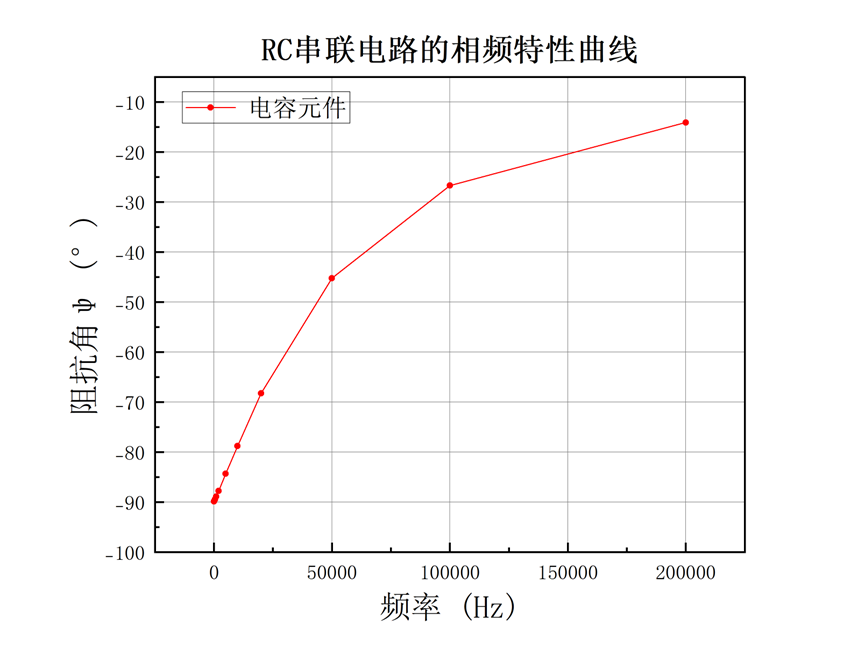
\includegraphics[width=0.55\linewidth]{RC.png}
	
	\label{}
\end{figure}
\textbf{图像关系:}

在RC串联电路中,阻抗的相位角是阻抗的虚部与实部的比值的反正切,定义为:

\[
\theta = \arctan\left( \frac{\Im(Z)}{\Re(Z)} \right),
\]

其中,\(Z = R + \frac{1}{j\omega C}\),
\( \omega = 2\pi f \) 为角频率,\(R\) 是电阻,\(C\) 是电容。

虚部和实部分别是:
- \(\Im(Z) = -\frac{1}{\omega C}\),
- \(\Re(Z) = R\).

因此,相位角可表示为:

\[
\theta = \arctan\left( -\frac{1}{\omega C R} \right).
\]

在低频条件下,\( \omega \) 很小,导致 \(-\frac{1}{\omega C}\) 很大,因此相位角接近 -90 度。

随着频率增大,\(\omega\) 增加,\(\frac{1}{\omega C}\) 减小,导致 \(-\frac{1}{\omega C R}\) 变小。这样,相位角开始增大并趋向于0,因为电阻的相对影响增加。

由于电阻 \(R\) 始终保持恒定,而电容的虚部随频率增大而减小,这使得相位角的增大过程较为平缓。随着频率进一步增大,实部的比重增加,虚部的影响减小,最终使相位角接近0。

因此,RC串联电路中的阻抗角从负90度随着频率增加而增大,并在高频时逐渐趋向于0。
\clearpage
\subsubsection{向量三角形和阻抗三角形}
根据实验数据,绘制给定分压比对应的频率点的电压向量三角形和阻抗三角形。
\begin{figure}[{H}]
	\centering
	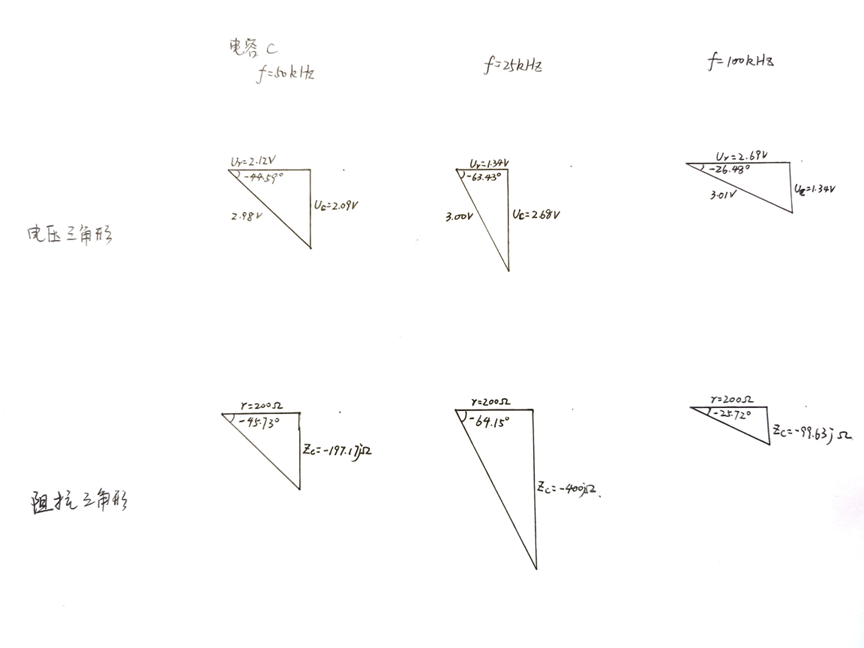
\includegraphics[width=0.6\linewidth]{三角形.png}
	\caption{电压向量三角形与阻抗三角形}
	\label{}
\end{figure}

\begin{table}[H]
    \centering
    \begin{tabular}{|c|c|c|c|}
        \hline
        分压比 & 测量值 (°) & 电压三角形 (°) & 相对误差 (\%) \\
        \hline
        1:1   & -45.73     & -44.59         & 2.56 \\
        1:2   & -64.15     & -63.43         & 1.13 \\
        2:1   & -25.72     & -26.48         &  2.87 \\
        \hline
    \end{tabular}
    \caption{相对误差}
\end{table}
相对误差较小,说明RC电路阻抗三角形和电压三角形在实际上对应同一个阻抗角符合图一所示的两种三角形相似。
\clearpage
\subsection{RL电路分析}
\subsubsection{幅频关系曲线}
根据实验数据,绘制幅频关系曲线
\begin{figure}[{H}]
	\centering
	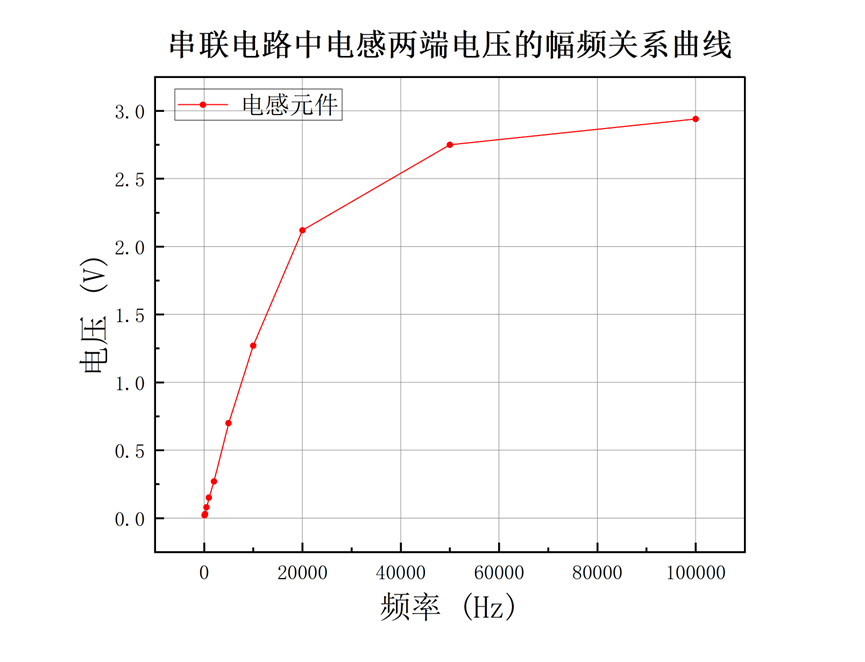
\includegraphics[width=0.4\linewidth]{l.png}
	
	\label{}
\end{figure}
\textbf{图像分析}

在RL串联电路中,电阻与电感串联连接,整个电路的总阻抗 \( Z \) 是两者的叠加,计算公式为:

\[
Z = R + j\omega L,
\]

其中,\( R \) 是电阻,\( L \) 是电感,\( \omega = 2\pi f \) 为角频率。

电感的阻抗,也称为感抗,随着频率增加而增大,其计算公式为:

\[
Z_L = j\omega L.
\]

在串联电路中,电压会根据阻抗的比例分配。电感两端的电压 \( V_L \) 可以通过分压公式计算:

\[
V_L = V_{in} \times \frac{Z_L}{R + Z_L}.
\]

将感抗代入得到:

\[
V_L = V_{in} \times \frac{j\omega L}{R + j\omega L}.
\]

随着频率增加,感抗 \( \omega L \) 变大,这导致电感在电路中所占的阻抗比例增加。根据分压公式,电感两端的电压随着频率增加而增大。

因此,RL串联电路中电感两端的电压随着频率增加而增加,是因为感抗与频率成正比,频率越高,电感在电路中所占的阻抗比重越大,导致分压增加。
\subsubsection{相频关系曲线}
根据实验数据绘制相频特性曲线
\begin{figure}[{H}]
	\centering
	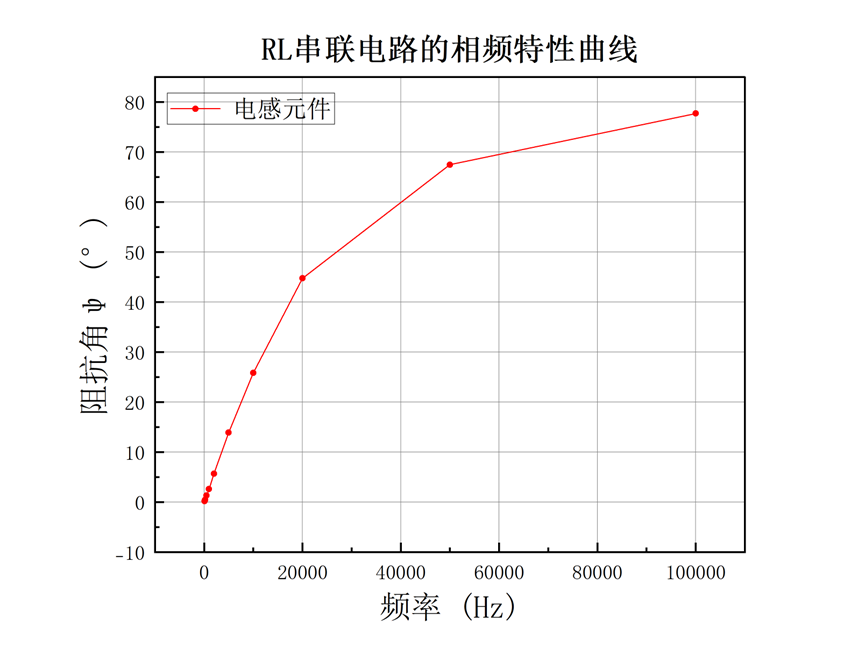
\includegraphics[width=0.4\linewidth]{RL.png}
	
	\label{}
\end{figure}
\textbf{图像分析:}

相位角的计算公式为:

\[
\theta = \arctan\left( \frac{\omega L}{R} \right).
\]

当频率较低时,虚部 \( \omega L \) 较小,实部 \( R \) 占主导地位,因此相位角 \(\theta\) 接近零度。

随着频率增加,虚部 \( \omega L \) 逐渐增加,而实部保持恒定。这导致虚部与实部的比值增大,相位角 \(\theta\) 随之增大。

因此,在RL串联电路中,阻抗角一开始接近零度,然后随着频率增高而逐渐增大。这是因为电感的感抗 \( \omega L \) 随着频率增加而增大,导致虚部占比增多,实部占比相对减少,从而使相位角逐渐增大。
\subsubsection{向量三角形和阻抗三角形}
根据实验数据,绘制给定分压比对应的频率点的电压向量三角形和阻抗三角形。
\begin{figure}[{H}]
	\centering
	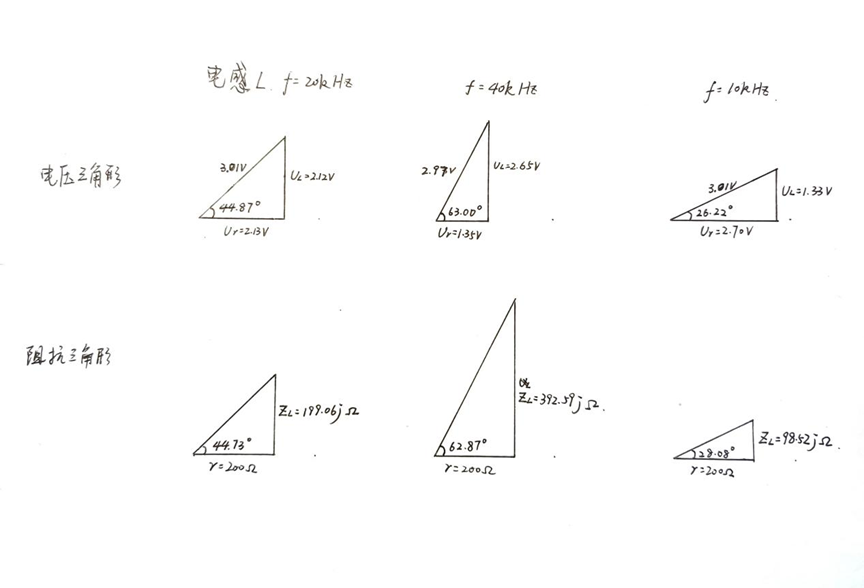
\includegraphics[width=0.7\linewidth]{三角形2.png}
	\caption{电压向量三角形与阻抗三角形}
	\label{}
\end{figure}

\begin{table}[H]
    \centering
    \begin{tabular}{|c|c|c|c|}
        \hline
        分压比 & 测量值 (°) & 电压三角形 (°) & 相对误差 (\%) \\
        \hline
        1:1   & 44.73      & 44.87             &  0.31 \\
        1:2   & 62.87      & 63                & 0.21 \\
        2:1   & 28.08      & 26.22             &  7.10 \\
        \hline
    \end{tabular}
    \caption{相对误差}
\end{table}

相对误差较小,说明RL电路的阻抗三角形和电压三角形在实际上对应同一个阻抗角符合图一所示的两种三角形相似。
	%
	\subsection{串联谐振电路}
	串联谐振电路(或串联 RLC 电路)是电阻(R)、电感(L)、和电容(C)串联连接的电路。当外部输入的信号频率达到特定值时,电路会发生谐振。谐振频率由电感和电容的特性决定,计算公式为 \( f_r = \frac{1}{2\pi \sqrt{L \cdot C}} \)。在这个频率下,电感和电容的电抗相互抵消,使得电路的总阻抗达到最小。
	\begin{figure}[{H}]
		\centering
		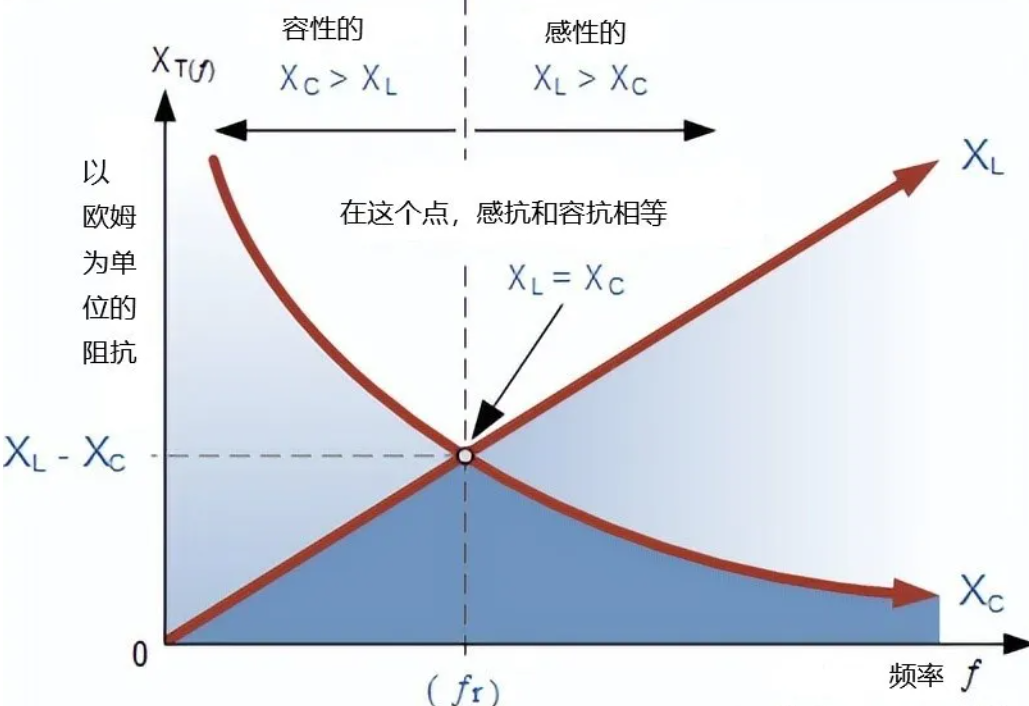
\includegraphics[width=0.6\linewidth]{串联谐振.png
		}
		\caption{串联谐振电路}
		\label{}
	\end{figure}

由于总阻抗最小,流过电路的电流在谐振频率时达到最大值,因此这个电路也被称为电流谐振电路。串联电路的总阻抗是电阻和电抗的平方和的平方根。在谐振频率时,电感和电容的电抗大小相等、符号相反,所以总阻抗等于电阻 \( Z = R \)。

在谐振时,电路的相位角为零,因为电感和电容的电抗相互抵消,电路的行为类似于纯电阻电路。相位角的计算公式为 \( \theta = \arctan\left( \frac{X_L - X_C}{R} \right) \)。

	
	%
	\subsection{计算L自有电阻}
	根据3.3中对于串联谐振电路的分析,本组设计测量方案时除直接测量法外,设计如图3所示电路,应用串联谐振的性质,当谐振时,电路内实际上有效电阻为纯电阻r与电感的自有电阻$R_L$,根据此实验原理对自有电阻进行测量。
	
	在实验电路中,我们设定电感为一个理想电感与自有电阻串联,然后计算此串联谐振电路的谐振频率为:
	$$f_{\mathrm{r}}=\frac1{2\pi\sqrt{\mathrm{LC}}}=5035HZ$$

	对此电路进行分析可以得出RL的计算公式为
	$$R_{L}=\frac{V}{V_{r}}\cdot r-r=27.97\Omega$$

	此结果与直接测量法所得结果($25.65\Omega$)较为接近,故认定此实验测量方法较为成功。
	%
	
	\clearpage
	
	% 小标题
	\section{ET6 R、L、C元件阻抗特性研究\quad\heiti 结语}
	% ---
	
	% 总结、杂谈与致谢
	\subsection{实验心得}
	\begin{enumerate}
		\item 实验中加深了我对于阻抗角的理解,对于课内知识有了具象化的印象。
		\item 实验中研究了关于串联谐振电路的相关知识,并设计了如报告中所示的实验方案对电感的自有电阻进行测量。
	\item \textbf{本实验报告采用LATEX编辑,实验分工为黄罗琳同学负责记录数据、编辑报告、数据分析,王显同学负责实验操作、误差分析、数据绘图。}
	\end{enumerate}
	\quad \large \textbf{感谢您对于此篇实验报告的阅读与批改,祝您工作顺利!}
	% ---
	

	% 附件
	\subsection{附件及实验相关的软硬件资料等}
	
	\begin{figure}[H]
		\centering
		\begin{minipage}[t]{0.45\textwidth}
			\centering
			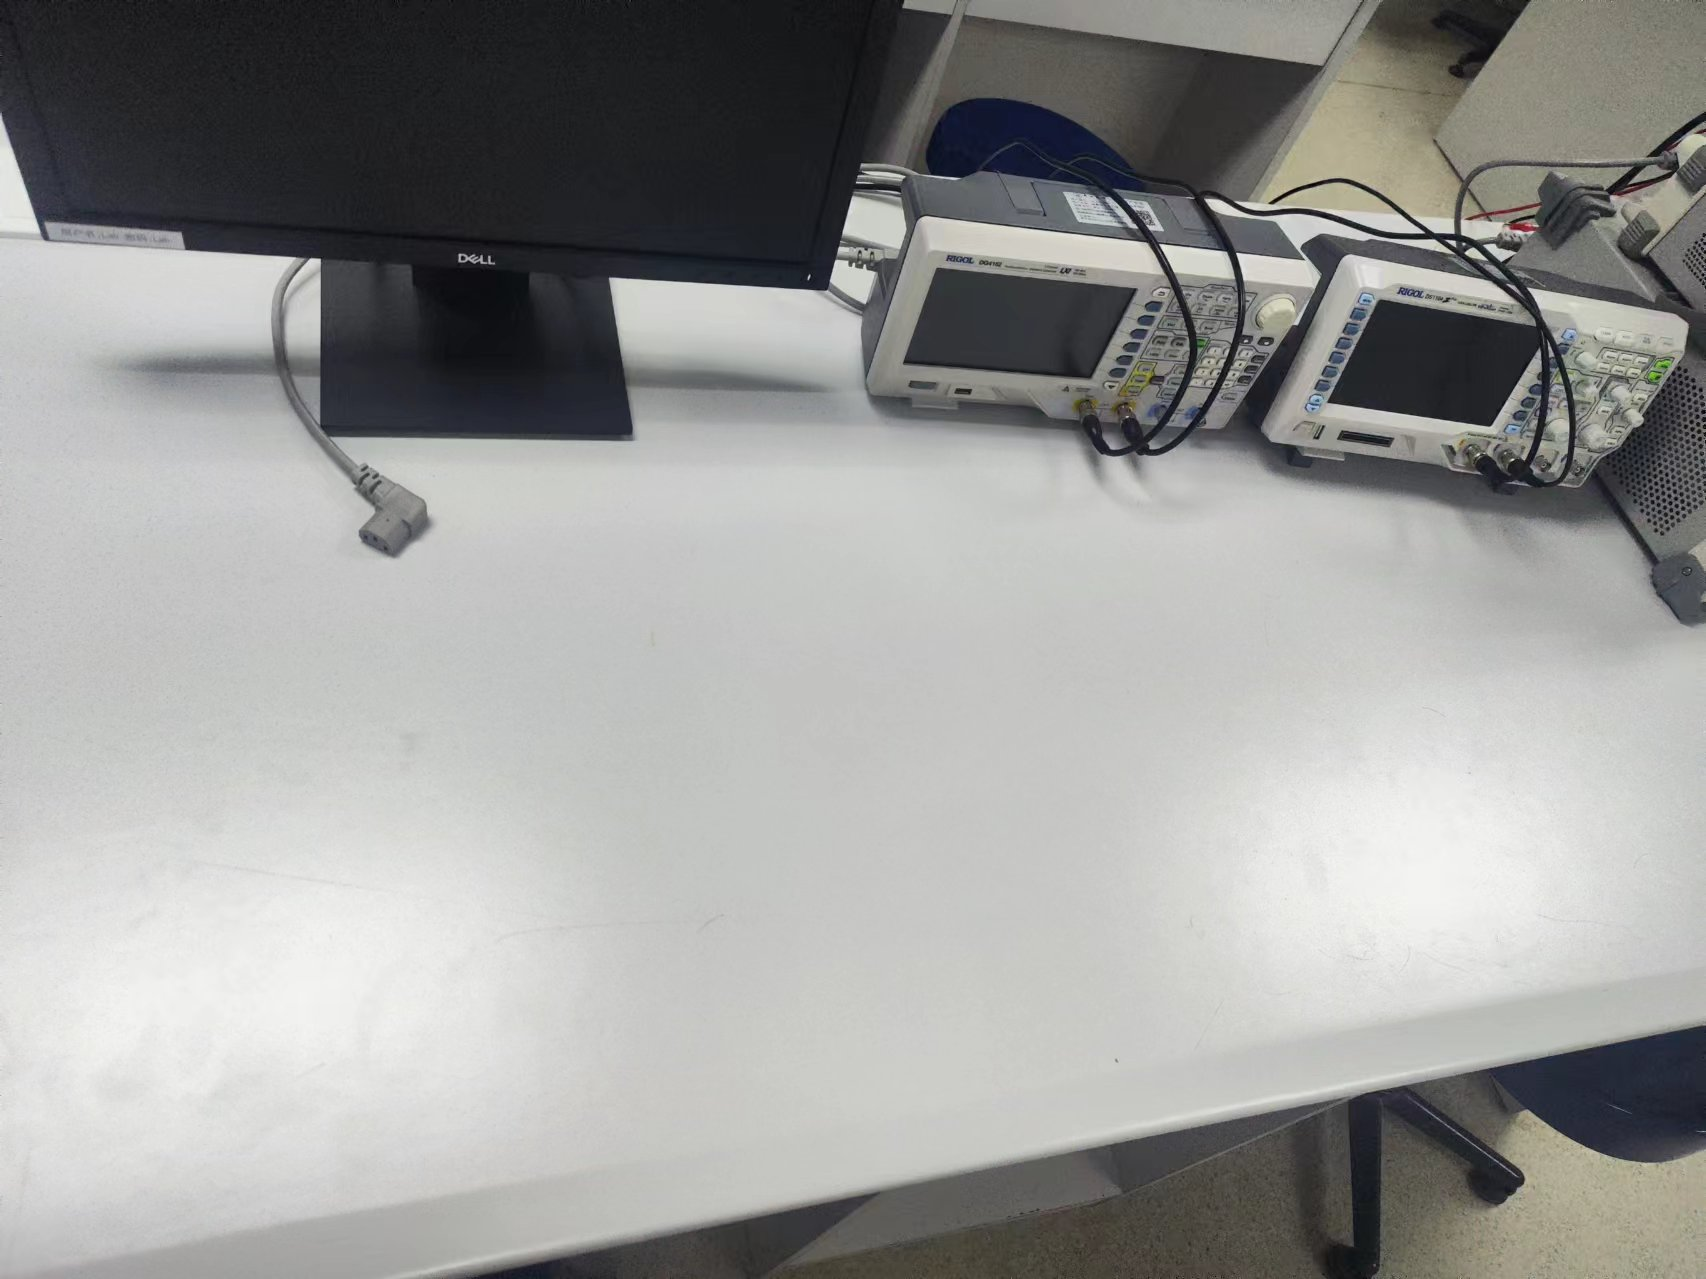
\includegraphics[width=0.8\linewidth]{桌面.jpg}
			\caption{实验桌面整理}
		\end{minipage}
		\hfill % 或使用 \quad 或 \hspace{5mm} 来控制间距
		\begin{minipage}[t]{0.45\textwidth}
			\centering
			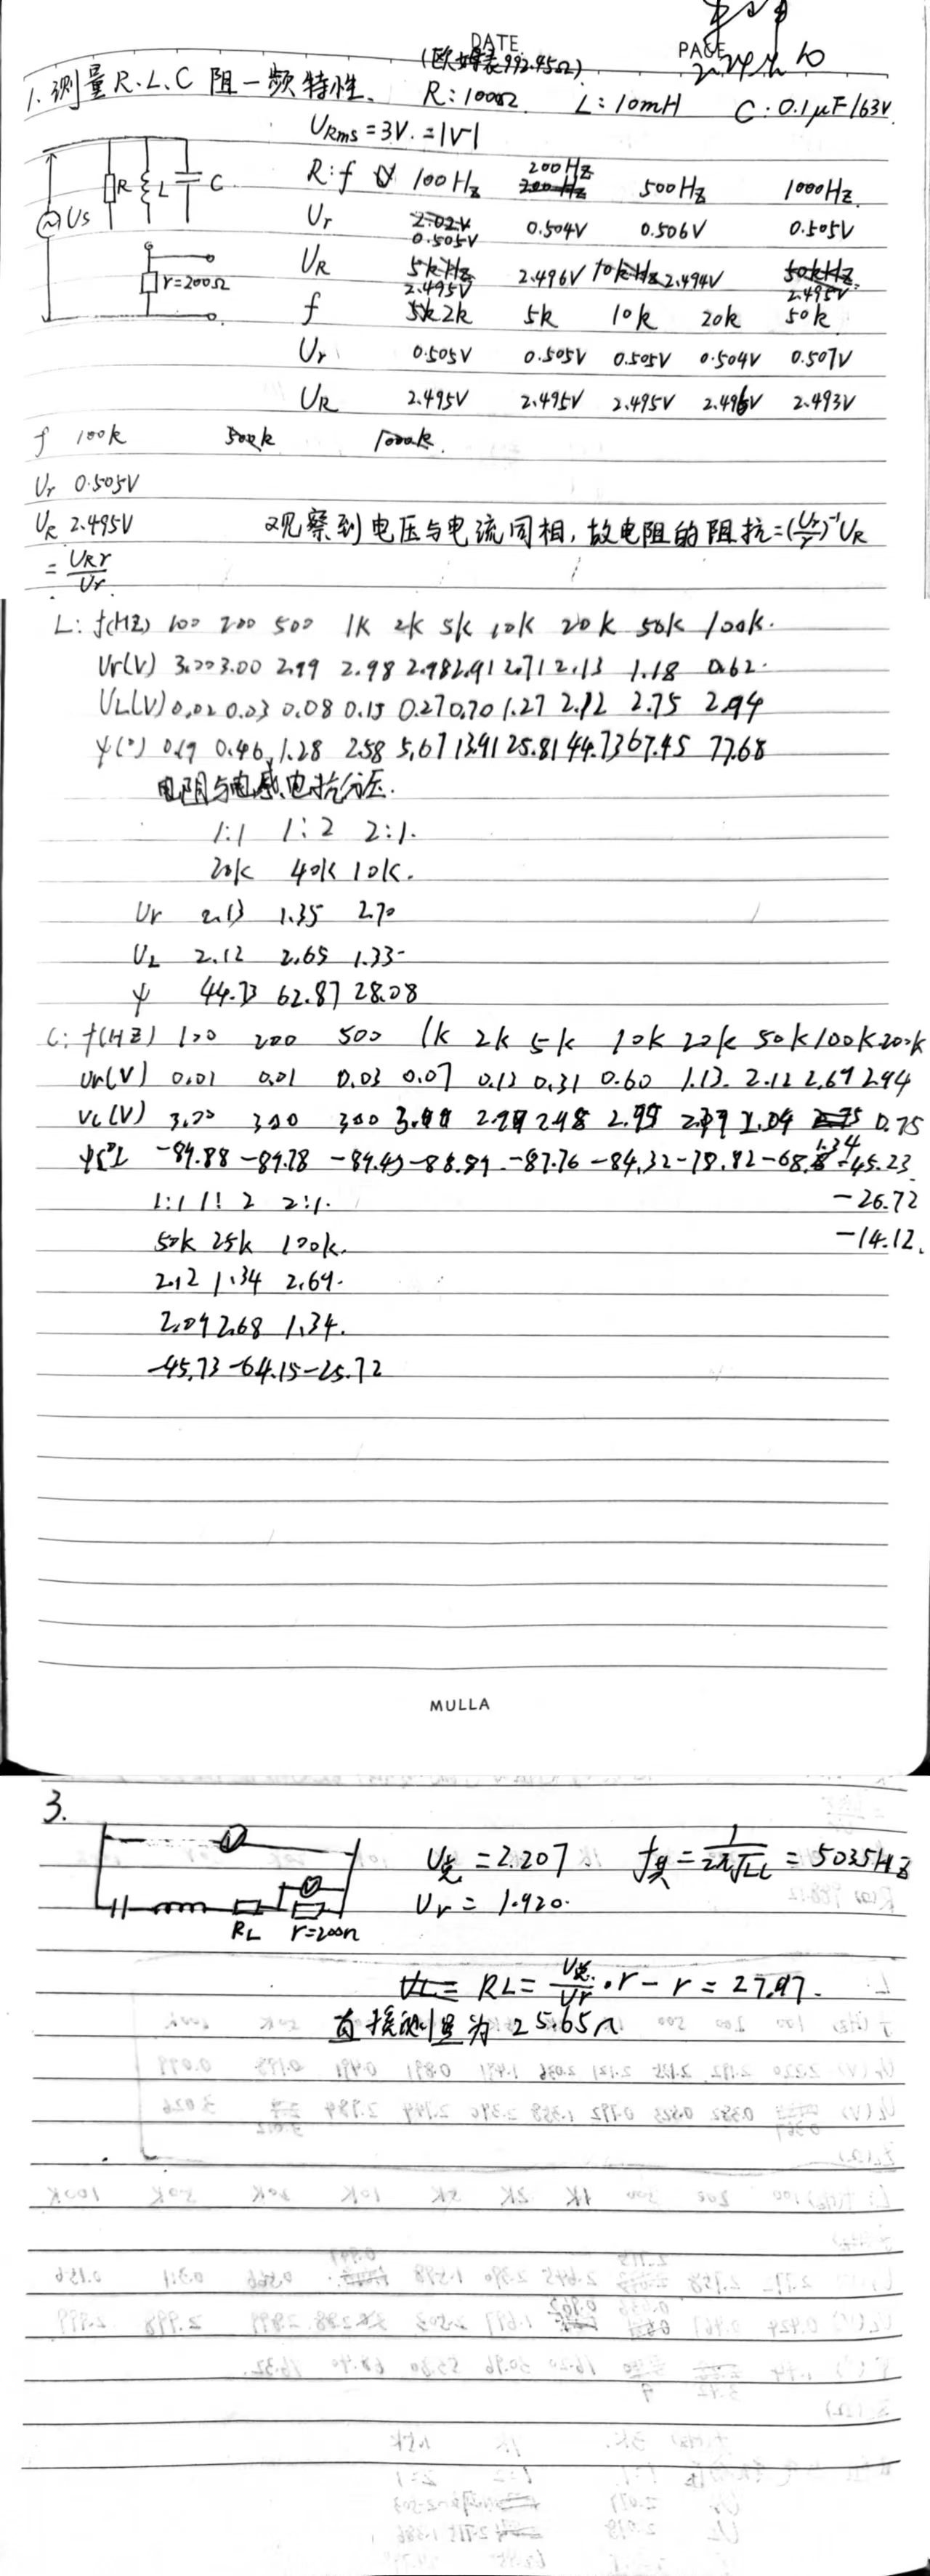
\includegraphics[width=0.5\linewidth]{数据.jpg}
			\caption{实验数据}
		\end{minipage}
	\end{figure}

	% ---
	
	
\end{document}